\documentclass[12pt]{article}
\setlength{\oddsidemargin}{0in}
\setlength{\evensidemargin}{0in}
\setlength{\textwidth}{6.5in}
\setlength{\parindent}{0in}
\setlength{\parskip}{\baselineskip}

\usepackage{amsmath,amsfonts,amssymb,graphicx,enumerate}

\begin{document}

CSCI 5454 \hfill Problem Set 2\\
Robert Werthman

\hrulefill

\begin{enumerate}

	\item \textit{Probability boot camp}
	
	\begin{enumerate}
	
		\item \textit{Prove Markov's inequality, $Pr[X \ge c] \le E[X]/c$, with $c>0$}\\
		\\
		The formula for the probability of a continuous random variable $X$ with probability density function $f(x)$ is
			$$
			Pr[x_1 \le X \le x_2] = \int_{x_1}^{x_2} f(x)dx
			$$	
		And the formula for the expected value of a continuous random variable $X$ with probability density function $f(x)$ is
			$$
			E[x_1 \le X \le x_2] = \int_{x_1}^{x_2} xf(x)
			$$	
		so for $Pr[X \ge c]$ we have
			$$
			Pr[X \ge c] = \int_{c}^{\infty} f(x)dx
			$$
		and since $X$ is a nonnegative random variable we have
			$$
			E[X] = \int_{0}^{\infty} xf(x)dx
			$$
		Notice that $0 < c \le \infty$.  This tells us that the bounds of $E[X]$ are greater than $Pr[X \ge c]$.  We can break up the integral formed by $E[X]$ to create an inequality that 
		will begin to look similar to the integral of $Pr[X \ge c]$.
			\begin{align*}
				E[X] &= \int_{0}^{\infty} xf(x)dx\\
				&= \int_{0}^{c} xf(x)dx + \int_{c}^{\infty} xf(x)dx\\
				&\ge \int_{c}^{\infty} xf(x)dx\\
			\end{align*}
		We can assume that $x \ge c$ because $c$ is one of the bounds of the integral.  This means we can substitute $c$ for $x$.
			\begin{align*}
				 \int_{c}^{\infty} xf(x)dx \ge \int_{c}^{\infty} cf(x)dx \ge c\int_{c}^{\infty} f(x)dx
			\end{align*}
		We now have an equation for $E[X]$ that has $Pr[X \ge c]$.
			$$
			E[X] \ge c\int_{c}^{\infty} f(x)dx = cPr[X \ge c]
			$$
		Dividing both sides by $c$ gives us
			$$
			E[X]/c \ge Pr[X \ge c]
			$$
		which is Markov's inequality.  We have just shown that $Pr[X \ge c] \le E[X]/c$, with $c>0$ is true based on the probability and expected value of the continuous random variable $X$.
		
		\newpage
		\item \textit{Prove Chebyshev's inequality $Pr[|X-\mu| \ge c \cdot \sigma] \le 1/c^2$}\\
		\\
		If we let $k = (c \cdot \sigma)$ we have
			$$
			Pr[|X-\mu| \ge c \cdot \sigma] = Pr[|X-\mu| \ge k]
			$$
		One of the properties of $|a|$ is that it can also be represented as $\sqrt{a^2}$ so we can change\\
			$$
			Pr[|X-\mu| \ge k] = Pr[\sqrt{(X-\mu)^2} \ge k]
			$$
		If we take the square root of both sides of the inequality we get
			$$
			Pr[(X-\mu)^2 \ge k^2]
			$$
		From here we can use Markov's inequality since we know $(X-\mu)^2$ is nonnegative.  If we let $(X-\mu)^2 = X$ and $k^2 = c$ and substitute those into Markov's inequality we have 
			$$
			Pr[(X-\mu)^2 \ge k^2] \le E[(X-\mu)^2]/k
			$$
		The variance $\sigma^2$ of a continuous random variable $X$ with mean $\mu$ is 
			$$
			\sigma^2 = E[(X-\mu)^2]
			$$
		So
			$$
			Pr[(X-\mu)^2 \ge k^2] \le E[(X-\mu)^2]/k
			$$
		Now becomes
			$$
			Pr[(X-\mu)^2 \ge k^2] \le \sigma^2/k
			$$
		If we now change $k$ back to $c \cdot \sigma$ we have the equation
			$$
			Pr[(X-\mu)^2 \ge (c \cdot \sigma)^2] \le \sigma^2/c^2 \cdot \sigma^2
			$$
		Reducing the right side of the equation results in
			$$
			Pr[(X-\mu)^2 \ge (c \cdot \sigma)^2] \le 1/c^2
			$$
		And taking the square root of both sides of the inequality on the left hand side of the equation results in
			$$
			Pr[\sqrt{(X-\mu)^2} \ge c \cdot \sigma] \le 1/c^2
			$$ 
		
		Which can be further reduced to 
			$$
			Pr[|X-\mu| \ge c \cdot \sigma] \le 1/c^2
			$$ 
		Which is Chebyshev's inequality.  We have just shown that Chebyshev's inequality can be proven using Markov's Inequality.
		\newpage
		\item \textit{Show that for any discrete random variables $X,X',E[X] = E[E[X|X']]$.}\\
		\\
		If we let $Y = X'$ we have
			$$
			E[X] = E[E[X|Y]]
			$$
		The expected value of a discrete random variable X is
			$$
			E[X] = \sum_{x} x \cdot Pr[X=x]
			$$
		The conditional probability for any two discrete random variables $X,Y$ is defined to be 
			$$
			Pr[X=x|Y=y] = \frac{Pr[X=x \cap Y=y]}{Pr[Y=y]}
			$$
		The conditional expectation for any two discrete random variable $X,Y$ is defined to be
			$$
			E[X|Y=y] = \sum_{x} x \cdot Pr[X=x|Y=y]
			$$
		Given the above assertions
			\begin{align*}
				E[E[X|Y]] &= E[\sum_{x} x \cdot Pr[X=x|Y]]\\
				&=\sum_{y} [\sum_{x} x \cdot Pr[X=x|Y=y]] \cdot Pr[Y=y]\\
				&=\sum_{x} x \sum_{y} Pr[X=x|Y=y] \cdot Pr[Y=y]\\
				&=\sum_{x} x \cdot Pr[X=x]\\
				&=E[X]
			\end{align*}
		Sources I used to complete this problem:
		\begin{itemize}
			\item http://www.maths.qmul.ac.uk/~pettit/MTH5122/notes15.pdf
			\item https://en.wikipedia.org/wiki/Expected\_value
			\item https://math.stackexchange.com/questions/1353418/expected-value-proof-law-of-total-expectation
		\end{itemize}
		
		\newpage
		\item \textit{Prove by induction that $E[X_t] = 0$ for a martingale.}\\
		\\
		We want to show that in a martingale sequence the expected value for a random variable $X_{t+1}$ is the random variable $X_t$ before it.\\
		\\
		\textbf{Base case: }\\
		\\
		When $t=0$ with $X_0 = 0$ we have
			\begin{align*}
			E[X_1|X_0] &= \sum_{x} x \cdot Pr[X_1=x|X_0 = 0]\\
			&=0\\
			\end{align*}
		\textbf{Inductive step: }\\
		\\
		We showed that the base case $E[X_1|X_0] = 0$ is true.  Therefore, we can say that $E[X_2|X_1] = E[E[X_1|X0]] = 0$ no matter what $X_2$ is.   This leads to the equation
			$$
			E[X_t|X_0,...,X_{t-1}] = E[E[...E[X_{1}|X_{0}]]] = 0
			$$
		So by induction we have just shown that $E[X_t] = 0$.
		
	\end{enumerate}
	\newpage
	\item \textit{Give a graph $G$ with a source vertex $s$ and a set of edges $E_\pi$ to every vertex in $G$ such that the path from $s$ to $v$ is the shortest
	path but the set of the edges $E_\pi$ cannot be produced by running a breadth-first search on $G$.} \\
	\\
	\begin{figure}[h]
	\caption{Example of a graph where there exists a set of edges that are the shortest path between vertices but will not be found by a breadth first search.}
	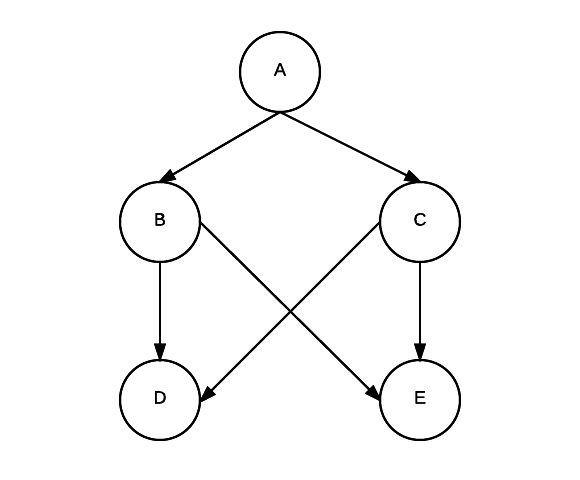
\includegraphics[width=6cm]{ps2_q2.png}
	\centering
	\end{figure}
	\\
	For this question, the shortest-path from $s$ to $v$ is defined as the minimum number of edges in any path from vertex $s$ to vertex $v$.  
	If we let the source vertex $s$ be vertex $A$ then the set of edges $E_\pi$ that cannot be produced by running a breadth first search are
	$$
	\{(A,B),(A,C),(B,D),(C,E)\}
	$$
	This is the case because of how breadth first search discovers vertices.  It starts at a source vertex $s$ and then adds every vertex in the adjacency list of $s$ to a queue.  
	In the case above $s$ will be $A$ and it will add $B$ and $C$ to the queue because those are the vertices adjacent to $A$.  
	An edge from $A$ to $B$ and from $A$ to $C$ will be created.  
	Once it does that it will then pop off the first vertex on the queue which will be either $B$ or $C$ depending on the ordering of the adjacency list of $A$.  
	It will then add every vertex from the adjacency list of the vertex is pops off to the queue.
	If either $B$ or $C$ is removed from the queue, $D$ and $E$ are still both added to the queue because there are both in $B$ and $C$ adjacency lists.
	In either case, edges are created from a single vertex, $C$ or $B$, to both $D$ and $E$ i.e. $(C,D),(C,E)$.  It will never be the case that both $C$ and $B$ will have a only single edge i.e. $(C,D),(B,E)$.
	It will only be the case that one of them will have two edges so the set of edges $E_\pi$ above will would never occur with a breadth first search.
	\newpage
	\item \textit{Give an efficient algorithm with an input of a graph $G$ and and an edge $e$ and returns a cut where $e$ is a light edge across the cut or NO if no such cut exists}\\
	\\
	\textbf{Psuedocode}
	\begin{verbatim}
	def LightEdgeCut(G,e):
	    minimum spanning tree = Kruskal's algorithm
	    if e is in minimum spanning tree:
	        create a cut of the graph with e as a light edge
	        return cut
	    else:
	        add e to minimum spanning tree to create a cycle C
	        z = largest edge removed from cycle C
	        if z is e: // Cycle property of minimum spanning tree
	            return NO
	        else:
	            create a cut of the graph with e as a light edge
	            return cut
	\end{verbatim}
	
	\textbf{Correctness}\\
	\\
	The algorithm above depends on two assumptions:
	\begin{enumerate}
		\item If an edge $(u, v)$ is contained in some minimum spanning tree, then it is a light edge crossing some cut of the graph [1].
		\item For any cycle C in the graph, if the weight of an edge e of C is larger than the individual weights of all other edges of C, then this edge cannot belong to a MST [2].
	\end{enumerate}
	As an example for hypothesis (a) we cut the the graph of Figure 2 between vertices $A$ and $D$ and vertices $D$ and $E$.  After the cut $S = \{D\}$ and $S'=\{A,B,C,E,F\}$.
	The edge $(A,D)$ is in the minimum spanning tree created by Kruskal's algorithm and it is a light edge of the cut that was made.\\
	\\
	As an example for hypothesis (b) if we add the edge $(D,E)$ to the minimum spanning tree it will create a cycle from vertices $A \rightarrow B \rightarrow E \rightarrow D \rightarrow A$.
	If we remove the largest weighted edge which in this case we say is $(A,D)$ even though it is the same weight as $(D,E)$ we get a new minimum spanning tree that has $(A,D)$ as an edge.  
	If $(A,D)$ had been larger than $(D,E)$ then it would have been removed from the minimum spanning tree and would not be part of any other minimum spanning tree.\\
	\\ 
	We assume Kruskal's algorithm is correct and returns a minimum spanning tree for the graph $G$.  
	It may be that the edge $e$ LightEdgeCut takes as input is part of the minimum spanning tree returned by Kruskal's algorithm.  
	We then know that the edge $e$ is a light edge crossing some cut of $G$ so we can create that cut with $e$ and return it. \\
	\\ 
	If $e$ is not in the minimum spanning tree returned by Kruskal's algorithm then we have to check to see if $e$ is part of any minimum spanning tree of $G$.
	We do this by adding it to the minimum spanning tree returned by Kruskal's algorithm in order to create a cycle.  
	Based on the cycle property of minimum spanning trees the largest edge in a cycle cannot be part of any minimum spanning tree.  If $e$ is the largest edge
	in the cycle we know it is not part of a minimum spanning tree and therefore not a light edge crossing some cut of the graph.  If it is not the largest edge then
	we can conclude it is part of a minimum spanning tree and is a light edge crossing some cut of the graph.\\
	\begin{figure}[h]
	\caption{A graph where the edges of a minimum spanning tree created by Kruskal's algorithm are highlighted in green.}
	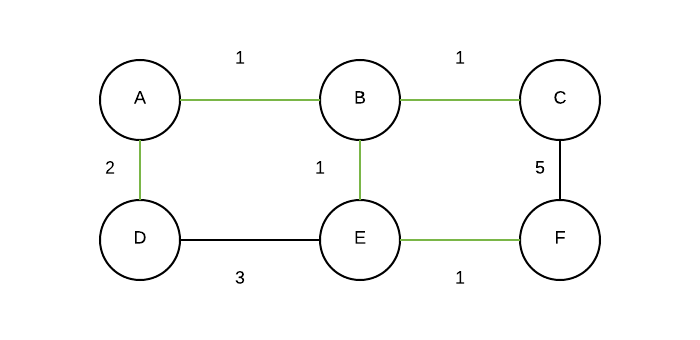
\includegraphics[width=8cm]{ps2_q3.png}
	\centering
	\end{figure}
	\\
	\textbf{Runtime}\\
	\\
	Kruskal's algorithm runs in $O(V\,log(E))$.  The worse case of this algorithm will, after going through Kruskal's algorithm, go to the else statement.
	Assuming the minimum spanning tree is a disjoint-set data structure adding the edge $e$ to the spanning tree is a set union operation that takes $O(1)$.
	Finding the edge with the highest weight in the cycle could take $O(V-1)$ if the cycle contains all of the edges in the minimum spanning tree.
	Checking if the largest edge is $e$ takes $O(1)$.  
	Creating a cut of the graph $G$ with $e$ as a light edge takes O(V) if it has to look at all of there vertices where to make the cut.
	The worst case runtime would be $O(V\,log(E)+V+(V-1)) = O(V\,log(E) + V)$.\\
	\\
	Sources I used to complete this problem.
	\begin{enumerate}[1]
		\item https://en.wikipedia.org/wiki/Minimum\_spanning\_tree
		\item http://test.scripts.psu.edu/users/d/j/djh300/cmpsc465/notes-4985903869437/solutions-to-some-homework-exercises-as-shared-with-students/4-solutions-clrs-23.pdf 
	\end{enumerate}
	
	\item


\end{enumerate}

\end{document}